\documentclass{beamer}
\usepackage{draculatheme}
\usepackage{bold-extra}
\usepackage{graphicx}  
\usepackage{tcolorbox}


\usepackage{pifont}
\usepackage{amsmath,amsthm} 
\usepackage{mathtools}
% \usepackage{arial}
\usepackage{amssymb}
\usepackage[framemethod=tikz]{mdframed}
\usepackage{tabularx}
\usepackage{mathrsfs}
\usepackage{multicol}
\usepackage{slashed}
\usepackage{enumerate}
\usepackage{enumitem}
\usepackage{lipsum} 
\usepackage{booktabs}   
\usepackage{ragged2e}
\usepackage{multirow}
\usepackage{caption}
\usepackage{listings}
% \usepackage{fourier}
% \usepackage{mathptmx}
\usepackage{helvet}
\definecolor{horange}{HTML}{f58026}
\hypersetup{
	colorlinks=true,
	linkcolor=horange,
	filecolor=horange,      
	urlcolor=horange,
}


%%% New Environments %%%
\newtheorem{exmp}{Example}[section]

%%% Custom Comands %%%

\newcommand{\cmark}{\ding{51}}%
\newcommand{\xmark}{\ding{55}}%

% Natural Numbers 
\newcommand{\N}{\ensuremath{\mathbb{N}}}

% Whole Numbers
\newcommand{\W}{\ensuremath{\mathbb{W}}}

% Integers
\newcommand{\Z}{\ensuremath{\mathbb{Z}}}

% Finite fields
\newcommand{\F}{\ensuremath{\mathbb{F}}}

% Rational Numbers
\newcommand{\Q}{\ensuremath{\mathbb{Q}}}

% Real Numbers
\newcommand{\R}{\ensuremath{\mathbb{R}}}

% Complex Numbers
\newcommand{\C}{\ensuremath{\mathbb{C}}}

\newcommand{\pfs}{\noindent\makebox[\linewidth]{\rule{\textwidth}{0.4pt}}\vspace{0.5cm}}
\definecolor{orangehdx}{rgb}{0.96, 0.51, 0.16}

% Normal colors
\definecolor{xred}{HTML}{BD4242}
\definecolor{xblue}{HTML}{4268BD}
\definecolor{xgreen}{HTML}{52B256}
\definecolor{xpurple}{HTML}{7F52B2}
\definecolor{xorange}{HTML}{FD9337}
\definecolor{xdotted}{HTML}{999999}
\definecolor{xgray}{HTML}{777777}
\definecolor{xcyan}{HTML}{80F5DC}
\definecolor{xpink}{HTML}{F690EA}
\definecolor{xgrayblue}{HTML}{49B095}
\definecolor{xgraycyan}{HTML}{5AA1B9}

% Dark colors
\colorlet{xdarkred}{red!85!black}
\colorlet{xdarkblue}{xblue!85!black}
\colorlet{xdarkgreen}{xgreen!85!black}
\colorlet{xdarkpurple}{xpurple!85!black}
\colorlet{xdarkorange}{xorange!85!black}
\definecolor{xdarkcyan}{HTML}{008B8B}
\colorlet{xdarkgray}{xgray!85!black}

% Very dark colors
\colorlet{xverydarkblue}{xblue!50!black}

% Document-specific colors
\colorlet{normaltextcolor}{black}
\colorlet{figtextcolor}{xblue}

% Light colors
\colorlet{xlightblue}{xblue!85!white}

% Enumerated colors
\colorlet{xcol0}{black}
\colorlet{xcol1}{xred}
\colorlet{xcol2}{xblue}
\colorlet{xcol3}{xgreen}
\colorlet{xcol4}{xpurple}
\colorlet{xcol5}{xorange}
\colorlet{xcol6}{xcyan}
\colorlet{xcol7}{xpink!75!black}

% Blue-Purple (should just used colorbrewer...)
\definecolor{xrainbow0}{HTML}{e41a1c}
\definecolor{xrainbow1}{HTML}{a24057}
\definecolor{xrainbow2}{HTML}{606692}
\definecolor{xrainbow3}{HTML}{3a85a8}
\definecolor{xrainbow4}{HTML}{42977e}
\definecolor{xrainbow5}{HTML}{4aaa54}
\definecolor{xrainbow6}{HTML}{629363}
\definecolor{xrainbow7}{HTML}{7e6e85}
\definecolor{xrainbow8}{HTML}{9c509b}
\definecolor{xrainbow9}{HTML}{c4625d}
\definecolor{xrainbow10}{HTML}{eb751f}
\definecolor{xrainbow11}{HTML}{ff9709}
\usepackage[T1]{fontenc} 







\usepackage{tikz}
\usetikzlibrary{shadows,shapes,backgrounds,calc,patterns}

\title{Quantum Cryptography}

\author[Beggs, Hill] % (optional, use only with lots of authors)
{P.~Beggs\inst{1} \and J.~Hill\inst{2}}
% - Give the names in the same order as the appear in the paper.
% - Use the \inst{?} command only if the authors have different
%   affiliation.

\institute%
{
  \inst{1}%
  Department of Astrology\\
  University of Southern Liberty in South Dakota
  \and
  \inst{2}%
  Department of Theoretical Physics\\
  Washington University in St.~Louis}



\date{\today}
\setbeamercolor{normal text}{fg=draculafg, bg=draculabg}
\setbeamercolor{alerted text}{fg=draculared}
\setbeamercolor{example text}{fg=draculagreen}
\setbeamercolor{structure}{fg=draculapurple}
\setbeamercolor{background canvas}{bg=draculabg}
\setbeamercolor{frametitle}{fg=draculafg, bg=draculacl}
\setbeamercolor{title}{fg=draculafg, bg=draculacl}
\setbeamerfont{title}{size=\huge, series=\bfseries}
\setbeamerfont{frametitle}{size=\Large, series=\bfseries}


\begin{document}

\begin{frame}[plain]
	\begin{tikzpicture}[overlay, remember picture]
		\node[fill=draculacl, drop shadow={fill=draculapurple}, rounded corners=5pt, inner sep=15pt, align=center] 
		at ($(current page.north) + (0,-2cm)$) {%
			\huge \textbf{\inserttitle} % Title inside the box
		};
	\end{tikzpicture}

    % Author, affiliation, and date below the title box
    \vspace{2cm} % Adjust vertical spacing as needed
    \begin{center}
        \large \insertauthor \\[1em]
        \small \insertinstitute \\[1em]
        \normalsize \insertdate
    \end{center}
\end{frame}

\begin{frame}
\frametitle{Introduction}
Content of the first slide. \\
% \begin{center}
% 	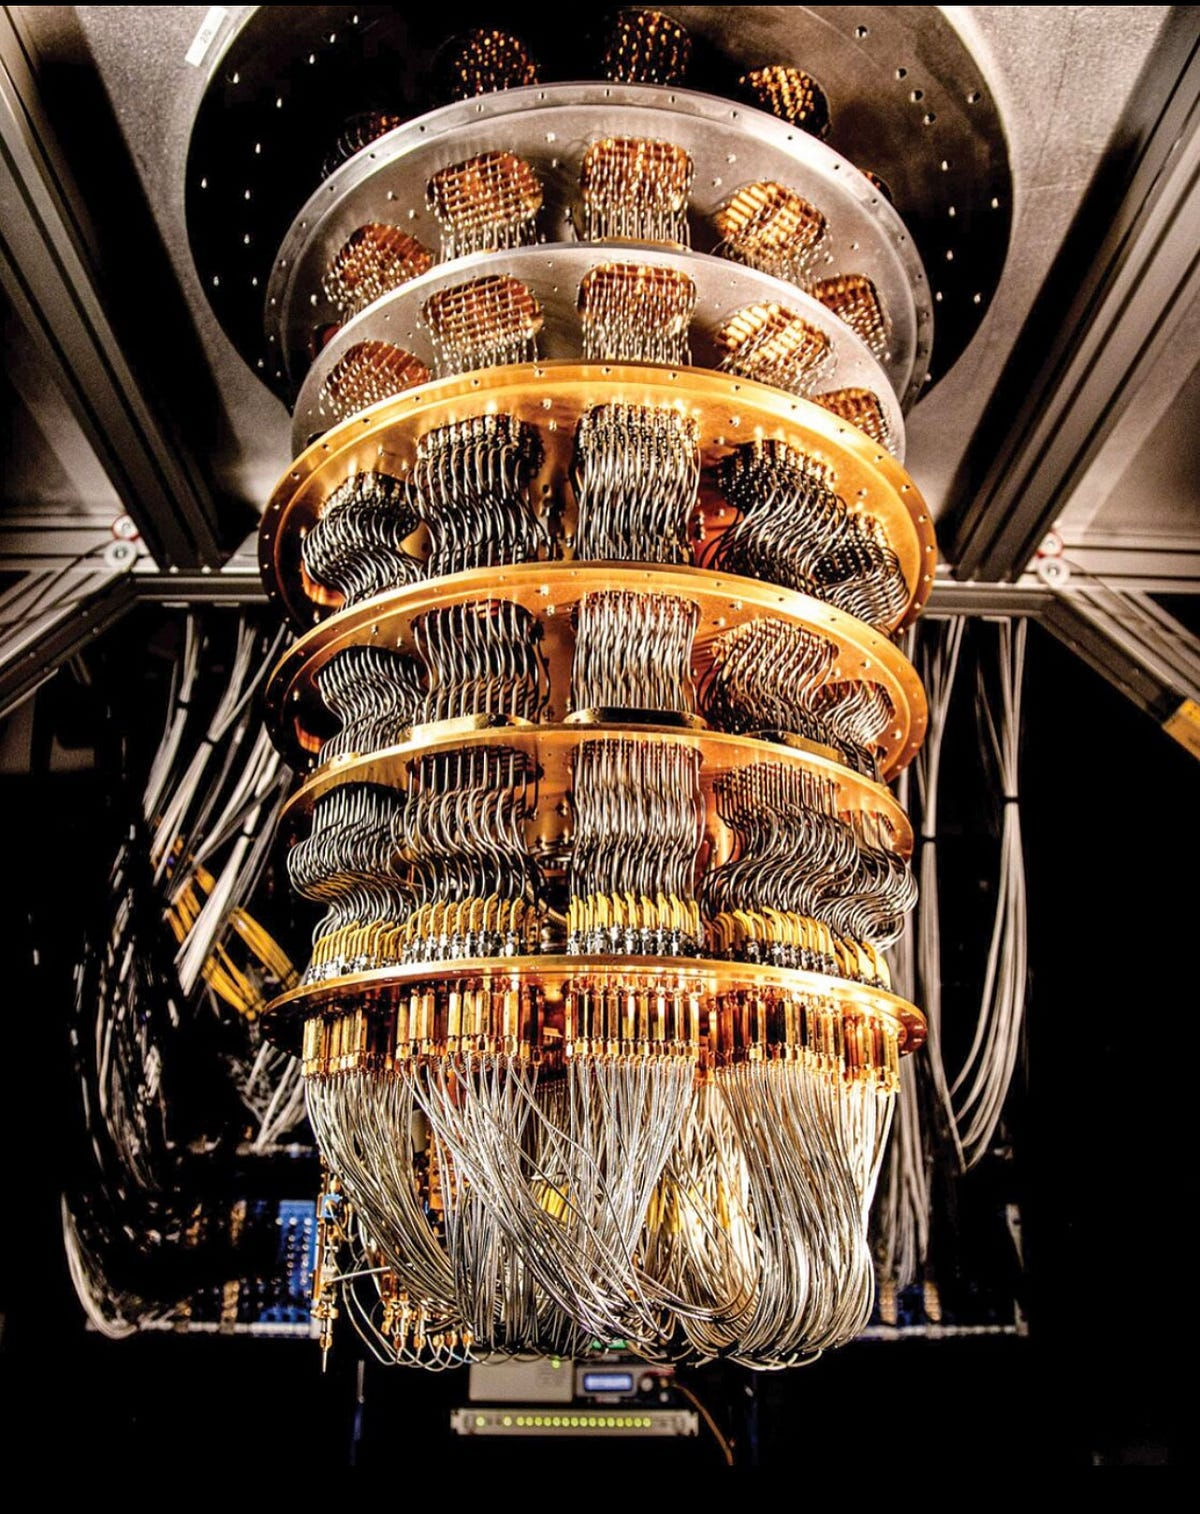
\includegraphics[height=5.5cm]{images/quantum_computer.jpg}	
% \end{center}

\begin{figure}
	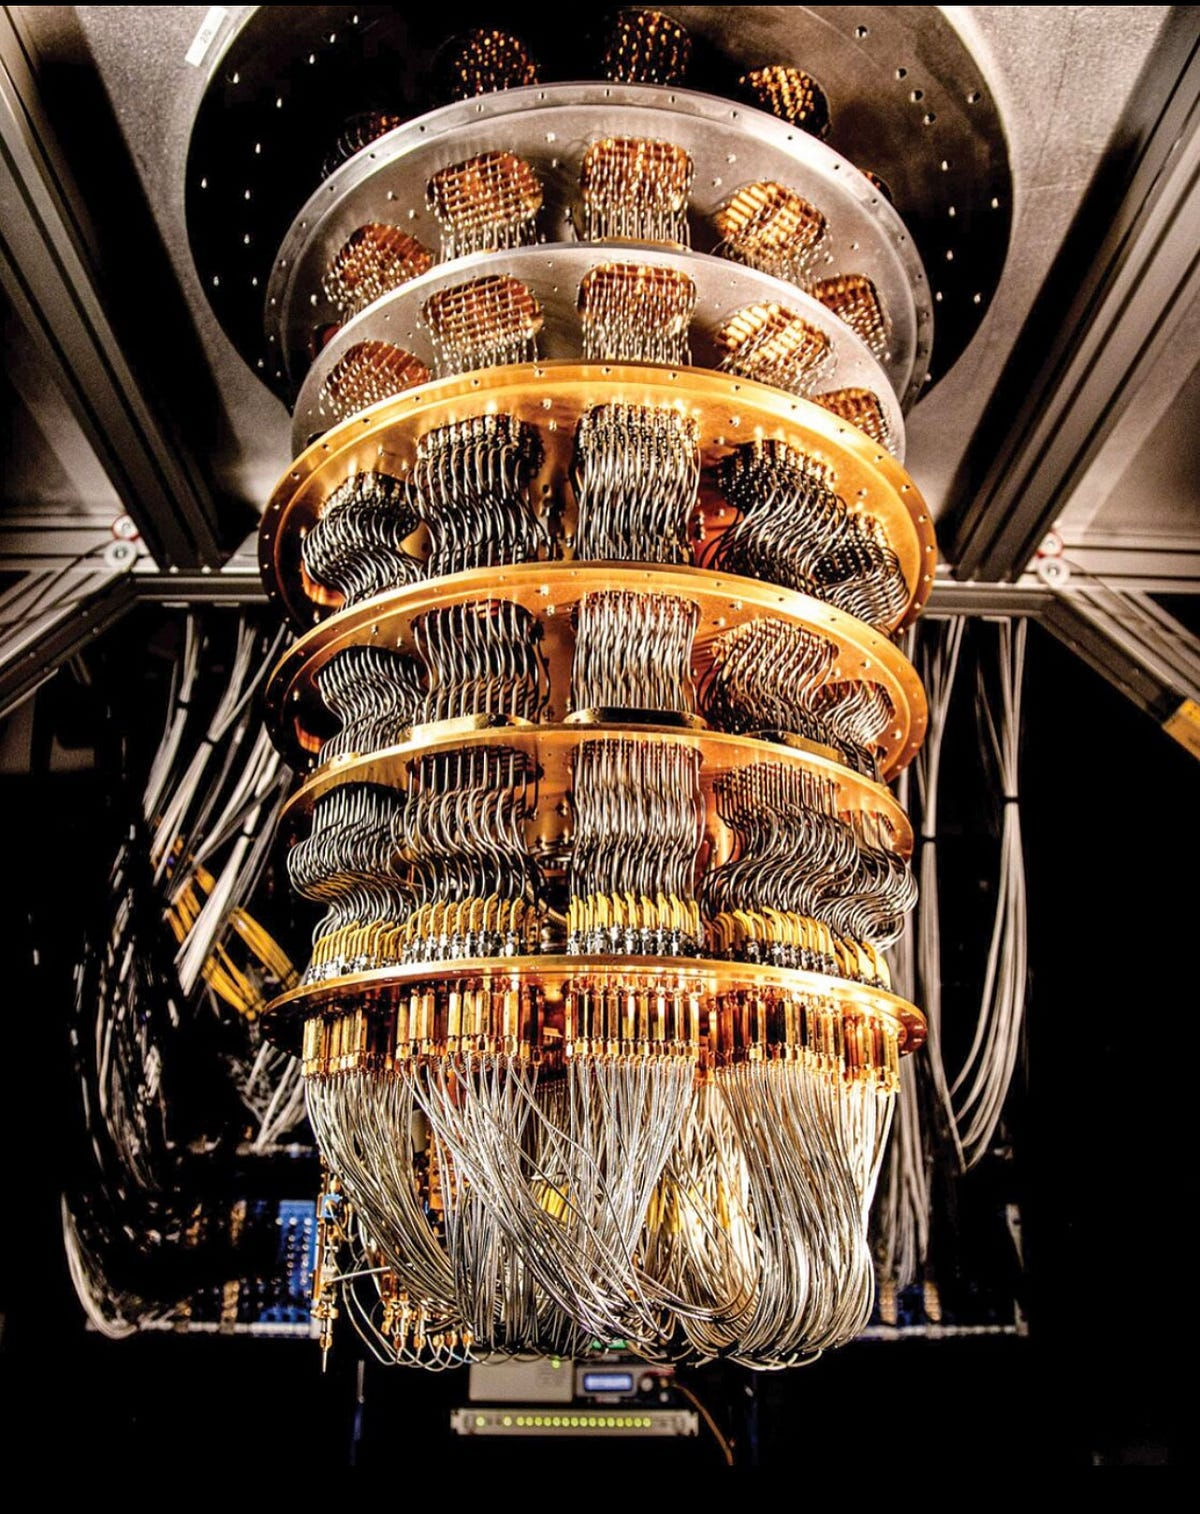
\includegraphics[height=5.0cm]{images/quantum_computer.jpg}
	\caption{This is a quantum computer!}
\end{figure}
\end{frame}

\begin{frame}
	\frametitle{There Is No Largest Prime Number}
	\framesubtitle{The proof uses \textit{reductio ad absurdum}.}

	\begin{theorem}
		There is no largest prime number.
	\end{theorem}
	\begin{proof}
		\begin{enumerate}
			\item[1-] Suppose $p$ were the largest prime number.
			\item[2-] Let $q$ be the product of the first $p$ numbers.
			\item[3-] Then $q + 1$ is not divisible by any of them.
			\item[1-] But $q + 1$ is greater than $1$, thus divisible by some prime
			number not in the first $p$ numbers.\qedhere
			\end{enumerate}
			\only[4-]{The proof used \textit{reductio ad absurdum}.}
	\end{proof}
	\alert{your mom smells}
\end{frame}


\end{document}
